\refstepcounter{Exercise}
\clearpage\subsection*{\theExercise CGIを使ってOpenJtalkに読み上げをさせよう}
\addtocounter{Exercise}{-1}\refstepcounter{Exercise}\label{E:Jtalk}
考え方

ウェブページから読み上げさせたい文章を受け取って、OpenJtalkにCGIから読み上げをさせよう。

まずは、試してみよう。

ブラウザを開いて

localhost:3000/jtalk.html

にアクセスをしてみよう。

%
%ぶらうざで開いた画面n
%koyaman
%September 20, 2019 2:50 AM


\centering
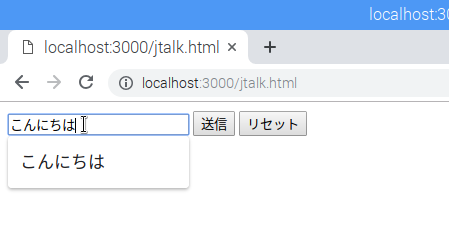
\includegraphics[width=0.85\textwidth]{ome7-img056.png}
\flushleft

テキストボックスに読み上げさせたい文章を入れて送信をしてみよう。送信を押すとCGIプログラムへ文章が送られ、OpenJtalkで音声合成をします。


\bigskip

結果をウェブページのaudioタグ(音声を再生するタグ)へ渡して\ruby{再生}{さいせい}をします。

%
%
%音声ファイルを再生する画面のスクショ
%koyaman
%September 20, 2019 2:50 AM


\centering
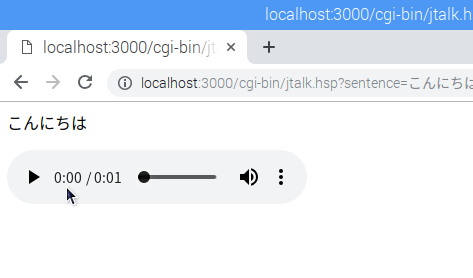
\includegraphics[width=0.85\textwidth]{ome7-img057.png}
\flushleft

\clearpage
プログラム解説

{\textasciitilde}/07/www/jtalk.html



\centering
\begin{boxedminipage}{16.148cm}
	\begin{enumerate}
	\baselineskip 10pt
	\setlength{\itemsep}{0cm}
	\item{\textless}!DOCTYPE html{\textgreater}

	\item{\textless}html{\textgreater}

	\item{\textless}head{\textgreater}

	\item\ \ \ \ {\textless}meta
	charset={\textquotedbl}utf-8{\textquotedbl}{\textgreater}

	\item{\textless}/head{\textgreater}

	\item{\textless}body{\textgreater}

	\item\ \ \ \ {\textless}form action={\textquotedbl}cgi-bin/jtalk.hsp{\textquotedbl}
	method={\textquotedbl}GET{\textquotedbl}{\textgreater}

	\item\ \ \ \ \ \ \ \ {\textless}input type={\textquotedbl}text{\textquotedbl}
	name={\textquotedbl}sentence{\textquotedbl}{\textgreater}

	\item\ \ \ \ \ \ \ \ {\textless}input type={\textquotedbl}submit{\textquotedbl}
	value={\textquotedbl}送信{\textquotedbl}{\textgreater}

	\item\ \ \ \ \ \ \ \ {\textless}input type={\textquotedbl}reset{\textquotedbl}
	value={\textquotedbl}リセット{\textquotedbl}{\textgreater}

	\item\ \ \ \ {\textless}/form{\textgreater}

	\item{\textless}/body{\textgreater}

	\item{\textless}/html{\textgreater}
	\end{enumerate}
\end{boxedminipage}
\flushleft
\bigskip


\bigskip


\bigskip



\bigskip

7〜11行目では、CGIようにフォーム(form)を用意しています。

文字を入れるテキストボックスが一つと送信用のボタンが一つ、テキストボックスをリセットするボタンが一つあります。

%
%スクリーンショット
%ブラウザでjtalk.htmlを開いた画像
%koyaman
%September 19, 2019 11:59 PM


7行目の

{\textless}form action={\textquotedbl}cgi-bin/jtalk.hsp{\textquotedbl}
method={\textquotedbl}GET{\textquotedbl}{\textgreater}

action=”cgi-bin/jtalk.hsp”

はフォームに入力された情報をを受ける(処理する)CGIプログラムを指定します。

method=”GET”

はクエリストリングとしてフォームの情報をCGIに渡すことを指示しています。

8行目の

{\textless}input type={\textquotedbl}text{\textquotedbl} name={\textquotedbl}sentence{\textquotedbl}{\textgreater}

では、テキストボックスを作っています。

name=”sentence”

はクエリストリングの名前を指定します。入力された文字列が値となります。ちなみにsentenceとは日本語にすると”文章”という意味になります。

例えば、テキストボックスに

“こんにちは”とテキストボックスに入力され、送信された場合

\clearpage
\bigskip



\centering
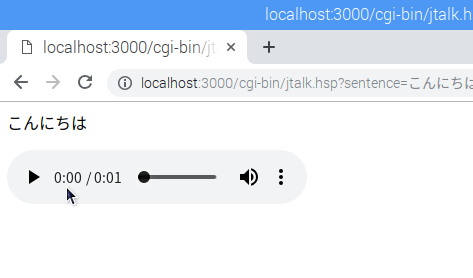
\includegraphics[width=0.85\textwidth]{ome7-img057.png}

\centering
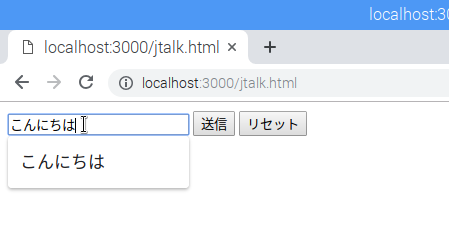
\includegraphics[width=0.85\textwidth]{ome7-img056.png}
\flushleft


\bigskip

%
%スクショ
%こんにちはとテキストボックスに
%koyaman
%September 20, 2019 12:04 AM


ウェブサーバにこのような要求を出します。

IPアドレス:3000/cgi-bin/jtalk.hsp?sentence=こんにちは

実際には”こんにちは”という文字列はURL内ではある\ruby{規則}{きそく}に\ruby{沿}{そ}って記号、数値に変換されています。

このことをパーセントエンコーディングといいます。CGIプログラムにクエリストリングが渡される前にウェブサーバは記号、数値に変換された文字列をもとに戻します。よって、プログラム内では入力された文字列と同じものを扱うことができます。

{\textasciitilde}/07/www/cgi-bin/jtalk.hsp

\centering
\begin{boxedminipage}{\textwidth}
	\begin{enumerate}
	\baselineskip 10pt
	\setlength{\itemsep}{0cm}
	\item \#include {\textquotedbl}hsp3cl.as{\textquotedbl}

	\item\#include {\textquotedbl}jtalk.as{\textquotedbl}

	\item\#include {\textquotedbl}cgi.as{\textquotedbl}

	\item

	\item mes {\textquotedbl}Content-type: text/html{\textbackslash}n{\textquotedbl}

	\item mes {\textquotedbl}{\textless}html{\textgreater}{\textless}head{\textgreater}{\textless}meta
	charset={\textbackslash}{\textquotedbl}utf-8{\textbackslash}{\textquotedbl}{\textgreater}{\textless}/head{\textgreater}{\textless}body{\textgreater}{\textquotedbl}


	\item

	\item getqueryval {\textquotedbl}sentence{\textquotedbl}, sentence

	\item jtsave sentence, wav\_file

	\item mes {\textquotedbl}{\textless}p{\textgreater}{\textquotedbl} + sentence +
	{\textquotedbl}{\textless}/p{\textgreater}{\textquotedbl}


	\item

	\item mes {\textquotedbl}{\textless}audio src={\textbackslash}{\textquotedbl}{\textquotedbl} \ + wav\_file +
	{\textquotedbl}{\textbackslash}{\textquotedbl}
	 type={\textbackslash}{\textquotedbl}audio/wav{\textbackslash}{\textquotedbl} controls{\textgreater}{\textquotedbl}

	\item mes {\textquotedbl}{\textless}/body{\textgreater}{\textless}/html{\textgreater}{\textquotedbl}

	\item end
	\end{enumerate}
\end{boxedminipage}
\flushleft

\bigskip

8行目でjtalk.htmlのフォームの

{\textless}input type={\textquotedbl}text{\textquotedbl} name={\textquotedbl}sentence{\textquotedbl}{\textgreater}

に入っている値を取り出しています。取り出した値はsentence変数へ入れています。

9行目の

jtsave sentence, wav\_file

はsentence変数の中の文字列を音声合成して音声ファイルのファイル名をwav\_file変数へ入れています。

12行目の

mes {\textquotedbl}{\textless}audio src={\textbackslash}{\textquotedbl}{\textquotedbl} \ + wav\_file +
{\textquotedbl}{\textbackslash}{\textquotedbl}
type={\textbackslash}{\textquotedbl}audio/wav{\textbackslash}{\textquotedbl} controls{\textgreater}{\textquotedbl}

	{\textless}audio{\textgreater}タグは音声ファイルを再生することができます。

src=”ファイル名”

では、再生するファイルを指定します。指定するファイルはドキュメントルート以下にないといけません。つまり、ドキュメントルートである{\textasciitilde}/07/wwwの中にある必要があります。

jtsave命令で作った音声ファイルは{\textasciitilde}/07/www/tmpの中にあります。ファイル名はwav\_file変数に入っています。

“
“の中で”を使うには{\textbackslash}”のように書きます。

type=”audio/wav”

では、音声ファイルの種類を決めます。jtsave命令が作る音声ファイルの場合は、

type=”audio/wav”にします。

controlsをつけると、再生ボタン、ミュートボタンなどが表示されます。

再生ボタンを押すと音声合成した音声ファイルが再生されます。

\clearpage
\refstepcounter{Question}\theQuestion\label{Q:Jtalk}

{\bfseries
	”おはようございます””こんばんは””ありがとうございます”を読ませてみよう。}


\bigskip

できる人は自分の自己紹介ページに({\textasciitilde}/07/www/index.html)に作ったフォームを変更して、こちらからCGIプログラムを起動するようにしましょう。

\ HINT: jtalk.htmlを参考にしてください。

\refstepcounter{Exercise}
\clearpage\subsection*{\theExercise CGIでセンサーの情報を表示させる}
\addtocounter{Exercise}{-1}\refstepcounter{Exercise}\label{E:Sensors}
考え方

温度、温度、\ruby{気圧}{きあつ}、照度センサーの情報をCGIを使ってウェブページから見れるようにしましょう。


\bigskip

まずは、プログラム実行してみましょう。

ブラウザを開いて、

localhost:3000/cgi-bin/sensors.hsp

にアクセスしてください。


%
%スクショ
%ブラウザで開いたときの
%koyaman
%September 20, 2019 2:37 AM


\centering
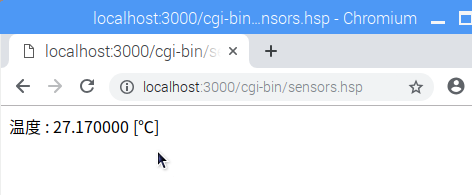
\includegraphics[width=0.75\textwidth]{ome7-img058.png}
\flushleft


温度センサーの値が表示されていると思います。

リロードするたびに値が更新されます。

今は温度センサーしか表示をしていないので、他のセンサーの値も表示させるように変更してみましょう。

%
%その他のセンサーを表示させた完成図のスクショ
%koyaman
%September 20, 2019 2:45 AM


\centering
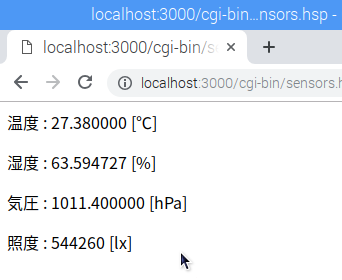
\includegraphics[width=0.75\textwidth]{ome7-img059.png}
\flushleft

次にプログラムを見てみましょう。


\clearpage
プログラム解説



\centering
\begin{boxedminipage}{16.81cm}
	\begin{enumerate}
	\baselineskip 10pt
	\setlength{\itemsep}{0cm}
	\item\#include {\textquotedbl}rpz-gpio-cl.as{\textquotedbl}

	\item\#include {\textquotedbl}hsp3cl.as{\textquotedbl}

	\item

	\item mes {\textquotedbl}Content-type: text/html{\textbackslash}n{\textquotedbl}

	\item mes {\textquotedbl}{\textless}html{\textgreater}{\textless}head{\textgreater}{\textless}meta
	 charset={\textbackslash}{\textquotedbl}utf-8{\textbackslash}{\textquotedbl}{\textgreater}{\textless}/head{\textgreater}{\textless}body{\textgreater}{\textquotedbl}

	\item

	\item i2c\_ch\_bme\ = \ 0

	\item i2c\_ch\_tsl \ = \ 1

	\item

	\item fail \ = \ init\_bme(i2c\_ch\_bme)\ \ \ \ ; 温\ruby{湿}{しつ}度気圧センサ bm280を初期化する

	\item if fail \{\ \ \ \ \ \ \ \ \ \ \ \   ; 初期化成功チェック

	\item\ \ mes {\textquotedbl}failed to init bme: {\textquotedbl} + fail

	\item\ \ end

	\item\}

	\item

	\item init\_lux i2c\_ch\_tsl\ \ \ \ \ \ ; 照度センサ tsl2572を初期化する

	\item

	\item*main

	\item\ \ temp = get\_temp(i2c\_ch\_bme)\ \ \ \ ; 温度取得
	\item\ \ hum \ = get\_hum(i2c\_ch\_bme)\ \ \ \ ; 湿度取得
	\item\ \ press= get\_press(i2c\_ch\_bme)\ \ \ \ ; 気圧取得
	\item\ \ lux \ = get\_lux(i2c\_ch\_bme)\ \ \ \ ; 照度取得

	\item

	\item

	\item\ \ ; 取得したデータの表示

	\item\ \ mes {\textquotedbl}{\textless}p{\textgreater}温度 : {\textquotedbl} + temp + {\textquotedbl}
	[℃]{\textless}/p{\textgreater}{\textquotedbl}

	\item

	\item\ \ \ \ mes {\textquotedbl}{\textless}/body{\textgreater}{\textless}/html{\textgreater}{\textquotedbl}

	\item\ \ \ \ end
	\end{enumerate}
\end{boxedminipage}
\flushleft
この例題は{\textasciitilde}/03/sensors.hspをもとにしています。詳しい解説はそちらを参照してください。

19~22行目で温度、湿度、気圧、照度センサーから情報を取得しています。

結果はそれぞれtemp, hum, press,
lux変数へ入っています。

26行目で、温度センサーの値をpタグで表示しています。

\bigskip


\bigskip


\bigskip

\clearpage
\refstepcounter{Question}\theQuestion\label{Q:sensors}

友達のCGIへアクセスして、センサーの値を確認してみよう。

温度センサーと同様に、湿度、気圧、照度センサーの値も表示させてみましょう。

\begin{center}
	\begin{boxedminipage}{0.5\textwidth}
		localhost:3000/cgi-bin/sensors\_table.hsp
	\end{boxedminipage}
\end{center}

にブラウザでアクセスをしてみましょう。

温度センサーの値が表形式で表示されたと思います。

%
%スクショ
%実行画面
%localhost:3000/cgi{}-bin/sensors\_table.hsp
%koyaman
%September 20, 2019 2:44 AM


\centering
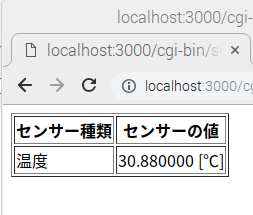
\includegraphics[width=0.8\textwidth]{ome7-img060.png}
\flushleft

次は、湿度、気圧、照度センサーの値を表形式で表示するように変更してみましょう。

\refstepcounter{Exercise}
\clearpage\subsection*{\theExercise 赤外線をウェブページから送信する}
\addtocounter{Exercise}{-1}\refstepcounter{Exercise}\label{E:IR}
CGIを使ってウェブページから赤外線を送信できるようにしましょう。

まずは、サンプルを動かしてみましょう。

ウェブブラウザを開いて

localhost:3000/ir.html

を開きましょう。

%
%開いた画像
%
%koyaman
%September 20, 2019 4:01 AM


\centering
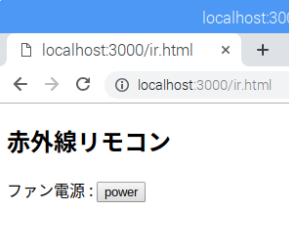
\includegraphics[width=17.006cm]{ome7-img061.png}
\flushleft

ボタンを押すとCGIで赤外線の送信をするコマンドが実行されます。

コマンドは、

irsend SEND\_ONCE fan onoff

が実行されます。リモコンの名前はfan、信号の名前はonoffになっています。

リモコンの名前、信号の名前が違う場合は、

{\textasciitilde}/07/www/cgi-bin/ir.hsp

を開いて

exec “irsend SEND\_ONCE fan onoff”

を変更して保存しましょう。

同じ場合はそのままで\ruby{大丈夫}{だいじょうぶ}です。

%
%スクショ
%ir.htmlのボタン
%koyaman
%September 20, 2019 4:05 AM


\centering
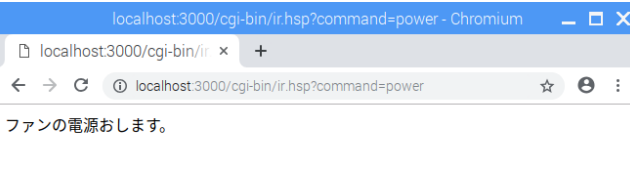
\includegraphics[width=16.671cm]{ome7-img062.png}
\flushleft

ブラウザのファン\ruby{電源}{でんげん}ボタンを押すと、CGIが起動して

赤外線を送信します。


\bigskip

\clearpage
プログラム解説

{\textasciitilde}/07/www/ir.html

8行目でフォームの\ruby{内容}{ないよう}を受け取るCGIを設定しています。

\centering
\begin{boxedminipage}{0.95\textwidth}
	\begin{enumerate}
	\baselineskip 10pt
	\setlength{\itemsep}{0cm}
	\item{\textless}!DOCTYPE html{\textgreater}

	\item{\textless}html{\textgreater}

	\item{\textless}head{\textgreater}

	\item\ \ \ \ {\textless}meta charset={\textquotedbl}utf-8{\textquotedbl}{\textgreater}

	\item{\textless}/head{\textgreater}

	\item{\textless}body{\textgreater}

	\item\ \ \ \ {\textless}h2{\textgreater}赤外線リモコン{\textless}/h2{\textgreater}

	\item\ \ \ \ {\textless}form action={\textquotedbl}cgi-bin/ir.hsp{\textquotedbl}
	method={\textquotedbl}GET{\textquotedbl}{\textgreater}

	\item\ \ \ \ \ \ \ \ {\textless}p{\textgreater}

	\item\ \ \ \ \ \ \ \ \ \ \ \ ファン電源 : {\textless}input type={\textquotedbl}submit{\textquotedbl}
	value={\textquotedbl}power{\textquotedbl} name={\textquotedbl}command{\textquotedbl}{\textgreater}

	\item\ \ \ \ \ \ \ \ {\textless}/p{\textgreater}

	\item\ \ \ \ {\textless}/form{\textgreater}

	\item{\textless}/body{\textgreater}

	\item{\textless}/html{\textgreater}
	\end{enumerate}
\end{boxedminipage}
\flushleft
{\textasciitilde}/07/www/cgi-bin/ir.hsp

がCGIとしてに起動します。

10行目で送信ボタンを作っています。

{\textless}input type={\textquotedbl}submit{\textquotedbl} value={\textquotedbl}power{\textquotedbl}
name={\textquotedbl}command{\textquotedbl}{\textgreater}

クエリストリングの名前はcommandで値はpowerとなります。このボタンが押されるとCGIが起動します。


\bigskip


\bigskip

\bigskip



\centering
\begin{boxedminipage}{16.36cm}
	\begin{enumerate}
	\baselineskip 10pt
	\setlength{\itemsep}{0cm}
	\item\#include {\textquotedbl}hsp3cl.as{\textquotedbl}

	\item\#include {\textquotedbl}cmdexec.as{\textquotedbl}

	\item\#include {\textquotedbl}cgi.as{\textquotedbl}


	\item

	\item mes {\textquotedbl}Content-type: text/html{\textbackslash}n{\textquotedbl}

	\item mes {\textquotedbl}{\textless}html{\textgreater}{\textless}head{\textgreater}{\textless}meta
	 charset={\textbackslash}{\textquotedbl}utf-8{\textbackslash}{\textquotedbl}{\textgreater}{\textless}/head{\textgreater}{\textless}body{\textgreater}{\textquotedbl}


	\item

	\item getqueryval {\textquotedbl}command{\textquotedbl}, cmd

	\item if cmd = {\textquotedbl}power{\textquotedbl} \{

	\item\ \ mes
		{\textquotedbl}{\textless}p{\textgreater}ファンの電源をおします。{\textless}/p{\textgreater}{\textquotedbl}

		\item\ \ exec {\textquotedbl}irsend SEND\_ONCE fan onoff{\textquotedbl}

		\item\} else \{

		\item\ \ \ \ mes
		{\textquotedbl}{\textless}p{\textgreater}コマンドが正しくありません{\textless}/p{\textgreater}{\textquotedbl}

		\item\ \ \ \ mes {\textquotedbl}{\textless}p{\textgreater}{\textquotedbl} + cmd +
	{\textquotedbl}{\textless}/p{\textgreater}{\textquotedbl}

	\item\}


	\item

	\item mes {\textquotedbl}{\textless}/body{\textgreater}{\textless}/html{\textgreater}{\textquotedbl}

	\item end
	\end{enumerate}
\end{boxedminipage}
\flushleft

\bigskip




\bigskip


\bigskip

8行目でクエリストリングから名前がcommandに対応する値を取り出してcmd変数へ入れています。

9〜15行目で受け取ったcmd変数をもとに条件判断をしています。cmdがpowerのときにファンの電源をつける赤外線を送っています。

それ以外の場合は正しいコマンドでないとして、メッセージを表示しています。


\bigskip

\bigskip
\refstepcounter{Question}\theQuestion\label{Q:IR}

ファンの電源をつける以外の赤外線送信機能を追加してみよう。

\ \ HINT :
まずは、ir.htmlにボタンを追加しよう。

\ \ \ \ そのあと、ir.hspの条件判断を追加しよう。

ir.htmlのフォームを自己紹介ページの一番下に付け加えよう。


\bigskip


\bigskip


\clearpage
CGIを使うときに便利なHSPの命令一覧

\begin{flushleft}
	\tablefirsthead{}
	\tablehead{}
	\tabletail{}
	\tablelasttail{}
	\begin{supertabular}{|m{5.467cm}|m{3.181cm}|m{7.7cm}|}
		\hline
		命令名/使い方 &
		例題 &
		効果\\\hline
		\#include “cgi.as”

		getqueryval “name”, var &
		\ref*{E:URL}

		\ref*{E:QS}

		\ref*{E:Jtalk}

		\ref*{E:IR} &
		クエリストリングから名前”name”を探して文字列として値を変数varへ入れる。

		\textbf{localhost:3000/cgi-bin/querystring.hsp?name=val}
		の場合、
		varにはvalが入る。\\\hline

		\#include “rpz-gpio-cl.as”
		cgpio 17, 1&
		\ref*{E:CGI}

		\ref*{E:QS}

		\ref*{E:Sensors} &
		gpio 命令と使い方は同じ。GPIO17 番に 1 を
		書き込む。gpio 命令との違いはプログラム終
		了時にも書き込んだ値が持続する。例えば、
		cgpio 17, 1 を実行すると、
		プログラム終了時でも 17 番の GPIO は 1 の
		ままになる。\\\hline

		\#include “rpz-gpio-cl.as”
		onoff = cgpioin(17)&
		\ref*{E:CGI} &
		gpio 命令と同じ。cgpio でプログラム終了時
		でも効果を持続させたい場合はこちらを使用
		する必要がある。\\\hline

		\#include “rpz-gpio-cl.as”&
		\ref*{E:CGI}

		\ref*{E:QS}

		\ref*{E:Sensors} &
		\#include “rpz-gpio.as”のコマンドライン\ruby{版}{ばん}
		コマンドラインや CGI で動くプログラムを書
		く場合はこちらを使う。cgpio, cgpioin 命令
		以外は同じ命令が使える。\\\hline

		\#include “jtalk.as”

		jtsave “こんにちは”, hello &
		\ref*{E:Jtalk} &
		“こんにちは”をOpenJtalkで音声合成をして、作った音声ファイルのファイル名をhello変数へ入れる。音声ファイルは/tmp/ディレクトリの下にランダムなファイル名で入る。

		例えば、hello変数の中身は

		“/tmp/tmp.abzgda”のような感じになる。 \\\hline
		end &
		すべての例題 &
		プログラムの終了を意味する。この命令はCGI用のプログラムを終了するときに必要。この命令がないとCGIのプログラムは終了しない。(ブラウザの読み込みが終わらなくなる。)\\\hline
	\end{supertabular}
\end{flushleft}

\bigskip

{\bfseries
	付録 ウェブサーバの停止方法}

電源を切る前、ウェブサーバが起動しているターミナルを\ruby{閉}{と}じる前、ウェブサーバを停止したいときは、ウェブサーバを起動したターミナル(./webserver.pyを実行している画面)を選択して


\bigskip

CtrlとCを同時に押します。


\bigskip

それでウェブサーバは終了します。


\bigskip


\bigskip


\bigskip
